%\begin{figure}[t]
%{\eightpoint
%\begin{verbatim}
%  int->int stateful filter SingleInductionFilter() {
%      int counter;
%      int max;
%  
%      work push 1 pop 1{
%
%          ...
%
%          counter = (counter + C);
%
%          if (counter > max) {
%              counter = 0;
%          } 
%      }
%  }
%\end{verbatim}
%\caption{Stateful StreamIt filter using induction variable state.\protect\label{fig:transform-before-simple}}}
%\end{figure}
%
%\begin{figure}[t]
%{\eightpoint
%\begin{verbatim}
%  int->int filter SingleInductionFilter() {
%      int max;
%  
%      work push 1 pop 1{
%          int counter = (iter() * C) % max;
%
%          ...
%
%      }
%  }
%\end{verbatim}
%\caption{Stateless StreamIt filter using iteration keyword.\protect\label{fig:transform-after-simple}}}
%\end{figure}
%
%
%\begin{figure}[t]
%{\eightpoint
%\begin{verbatim}
%  int->int stateful filter StartingValueInductionFilter() {
%      int counter;
%      int start;
%      int max;
%
%      init {
%          counter = start;
%      }
%  
%      work push 1 pop 1{
%
%          ...
%
%          counter = (counter + 1);
%
%          if (counter > max) {
%              counter = start;
%          } 
%      }
%  }
%\end{verbatim}
%\caption{Stateful StreamIt filter using induction variable state starting at and resetting to a special starting value.\protect\label{fig:transform-before-starting}}}
%\end{figure}
%
%\begin{figure}[t]
%{\eightpoint
%\begin{verbatim}
%  int->int filter StartingValueInductionFilter() {
%      int max;
%      int start;
%  
%      work push 1 pop 1{
%          int counter = iter() % (max - start) + start;
%
%          ...
%
%      }
%  }
%\end{verbatim}
%\caption{Stateless StreamIt filter using iteration keyword starting at and resetting to a special starting value.\protect\label{fig:transform-after-starting}}}
%\end{figure}
%
%\begin{figure}[t]
%{\eightpoint
%\begin{verbatim}
%  int->int stateful filter TwoNestedInductionFilter() {
%      int counter_x;
%      int counter_y;
%      int max_x;
%      int max_y;
%  
%      work push 1 pop 1{
%
%          ...
%
%          counter_x = (counter_x + 1);
%
%          if (counter_x > max_x) {
%              counter_x = 0;
%              counter_y = (counter_y + 1);
%
%              if (counter_y > max_y) {
%                  counter_y = 0
%              }
%          } 
%      }
%  }
%\end{verbatim}
%\caption{Stateful StreamIt filter using induction variable state starting at and resetting to a special starting value.\protect\label{fig:transform-before-twonested}}}
%\end{figure}
%
%\begin{figure}[t]
%{\eightpoint
%\begin{verbatim}
%  int->int filter TwoNestedInductionFilter() {
%      int max_x;
%      int max_y;
%    
%      work push 1 pop 1{
%          int counter_x = (iter() % max_x);
%          int counter_y = (iter() / max_x) % max_y;
%
%          ...
%
%      }
%  }
%\end{verbatim}
%\caption{Stateless StreamIt filter using iteration keyword starting at and resetting to a special starting value.\protect\label{fig:transform-after-twonested}}}
%\end{figure}

\section{The Iteration Keyword}
\label{sec:iteration}
We introduce a new language construct that maintains a value 
indicating how often the corresponding filter has been invoked.  
With the introduction of a new language construct, hereafter referred to as {\tt iter()}, the programmer can take measures to write their programs to expose data parallelism.  

\subsection{Language Construct Approach}
Syntactically, {\tt iter()} is equivalent to a field that is incremented on every {\tt prework} and {\tt work} invocation.  The value returned by {\tt iter()} indicates how often the filter has been invoked.  

Induction variable state requires the user to maintain mutable state, updating such state within the filter invocation, and potentially resetting them when required. The programmer can eliminate much of this code simply by arithmetically manipulating {\tt iter()} usage, as illustrated in Figures~\ref{fig:transform-after-simple} and~\ref{fig:transform-after-start}.  The implementation using {\tt iter()} describes the induction variable's full behavior much more succintly.  It is easy to lose track of where or what causes the induction variable to be updated, but the use of {\tt iter()} allows all of this information to be localized.

Multiple induction variables, as used with the stateful filter in Figure~\ref{fig:transform-after-twonested}, can be redefined in terms of {\tt iter()} as well.  It is not necessary to maintain multiple separate values for state.  Independent and nested induction variable state alike can be defined in terms of {\tt iter()}.

The transformations from filters using induction variable state to using {\tt iter()} are fairly simple for users to implement.  Many of these transformations simply require the user to translate their induction variables in terms how often the filter has been invoked.  User defined induction variables can all be derived from this value arithmetically.  

Some of the most common transformations used in the StreamIt benchmark suite can be summarized below.  
\begin{itemize}
\item Incrementing the induction variable by $C$ for each invocation scales the running value by $C$, as illustrated in Figure~\ref{fig:transform-after-simple}.

\item Placing an upper bound on the induction variable value establishes a range of values it may take.  This requires taking the running value modulo the size of this range, as illustrated in Figure~\ref{fig:transform-after-simple}.

\item Initializing and resetting the induction variable to a special starting value reduces the total range of values the induction variable can take.  The running value is taken modulo the size of this new range to calculate the current excess over the special starting value.  We add this value to the special starting value, as illustrated in Figure~\ref{fig:transform-after-start}.

\item A nested induction variable updates only when another induction variable reaches a certain threshold.  We scale the running value down according to this threshold to indicate it is incremented only once every time this threshold is reached by the other induction variable, as illustrated in Figure~\ref{fig:transform-after-twonested}.
\end{itemize}

\begin{figure}[t]
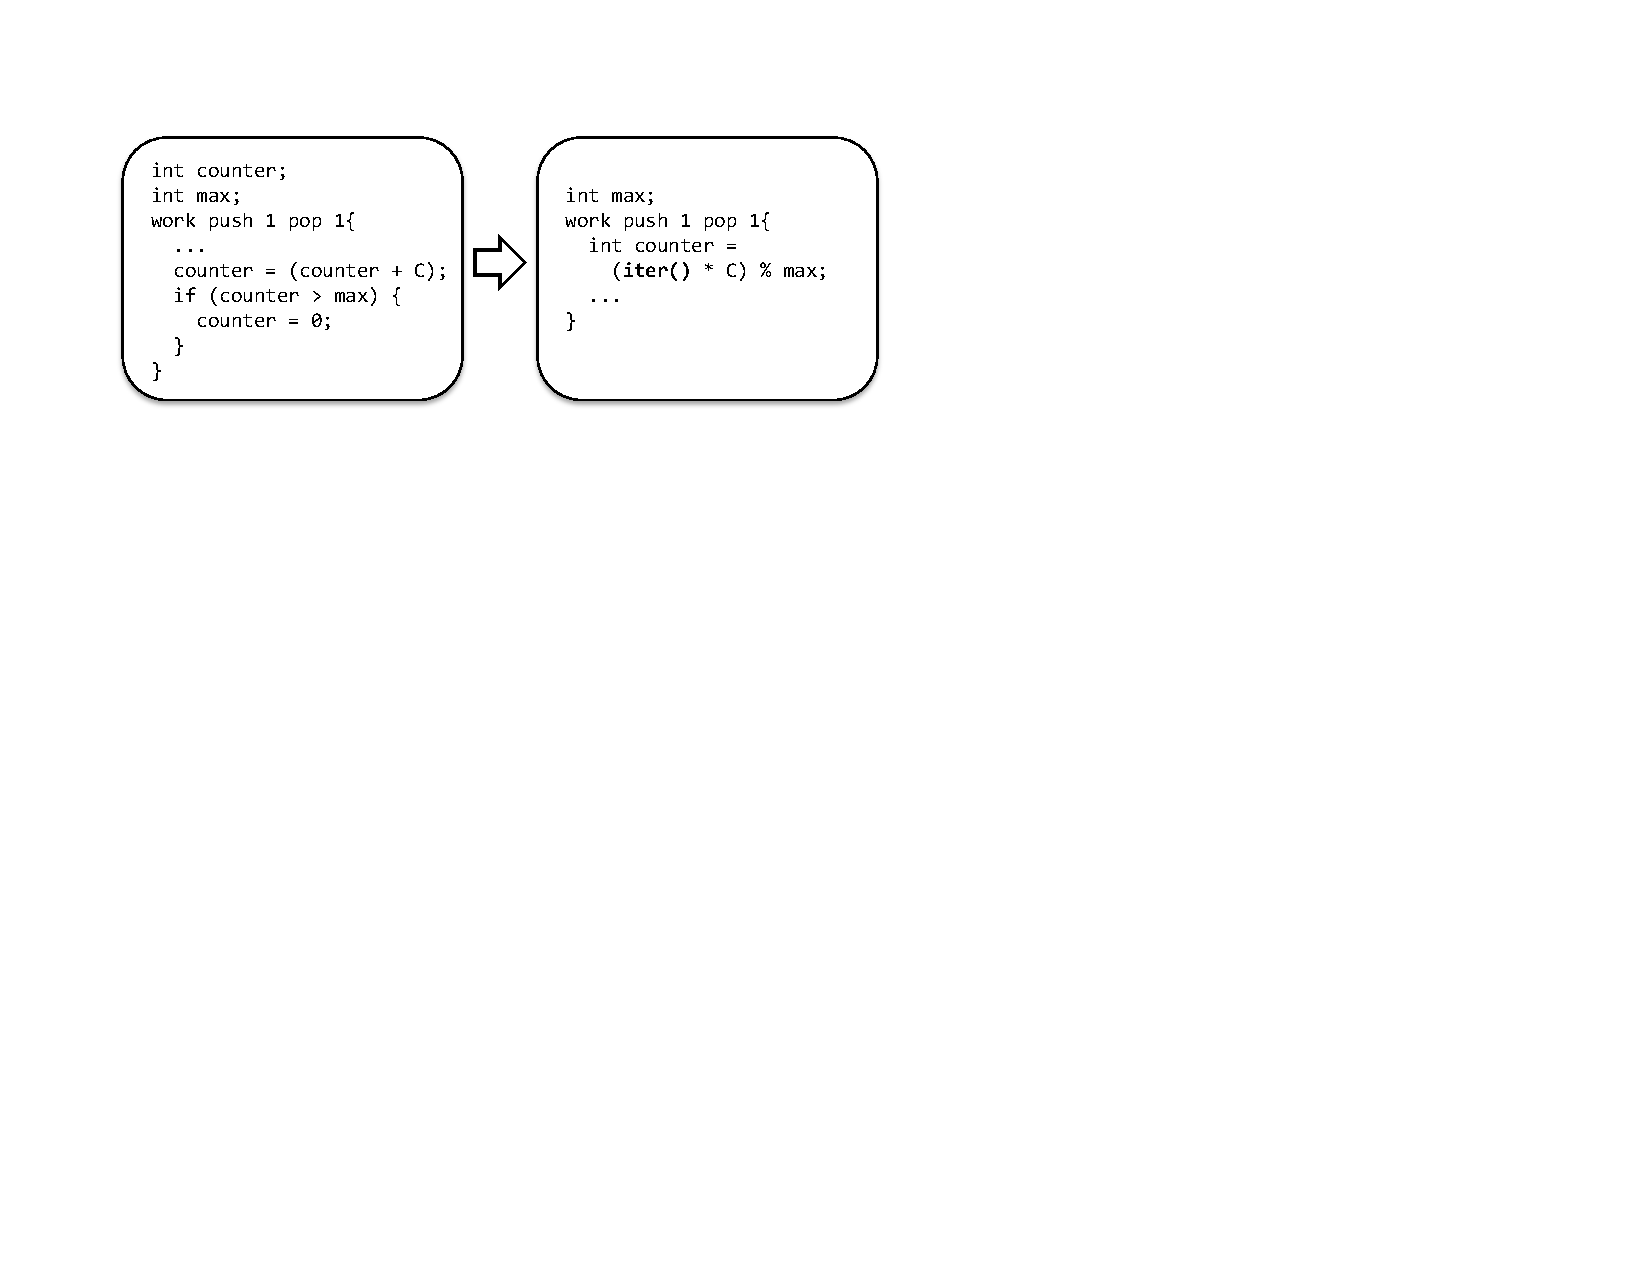
\includegraphics[width=3.3in]{figures/transformation1.pdf}
\caption{Translation of a simple filter with induction variable state that resets after a certain value. \protect\label{fig:transform-after-simple}}
\end{figure}

\begin{figure}[t]
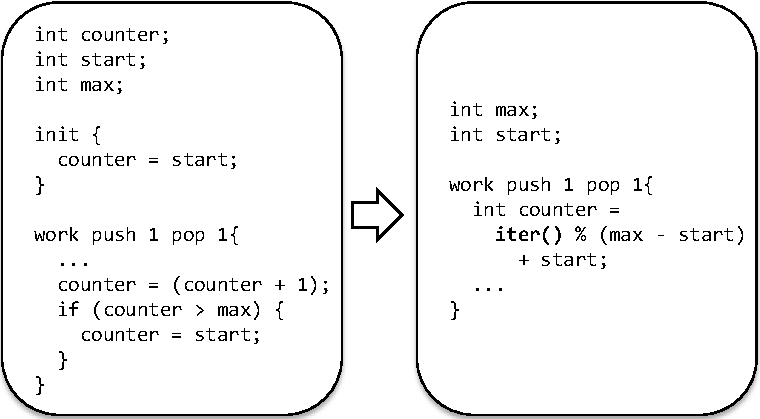
\includegraphics[width=3.3in]{figures/transformation2.pdf}
\caption{Translation of a simple filter with induction variable state that resets to a special value. \protect\label{fig:transform-after-start}}
\end{figure}

\begin{figure}[t]
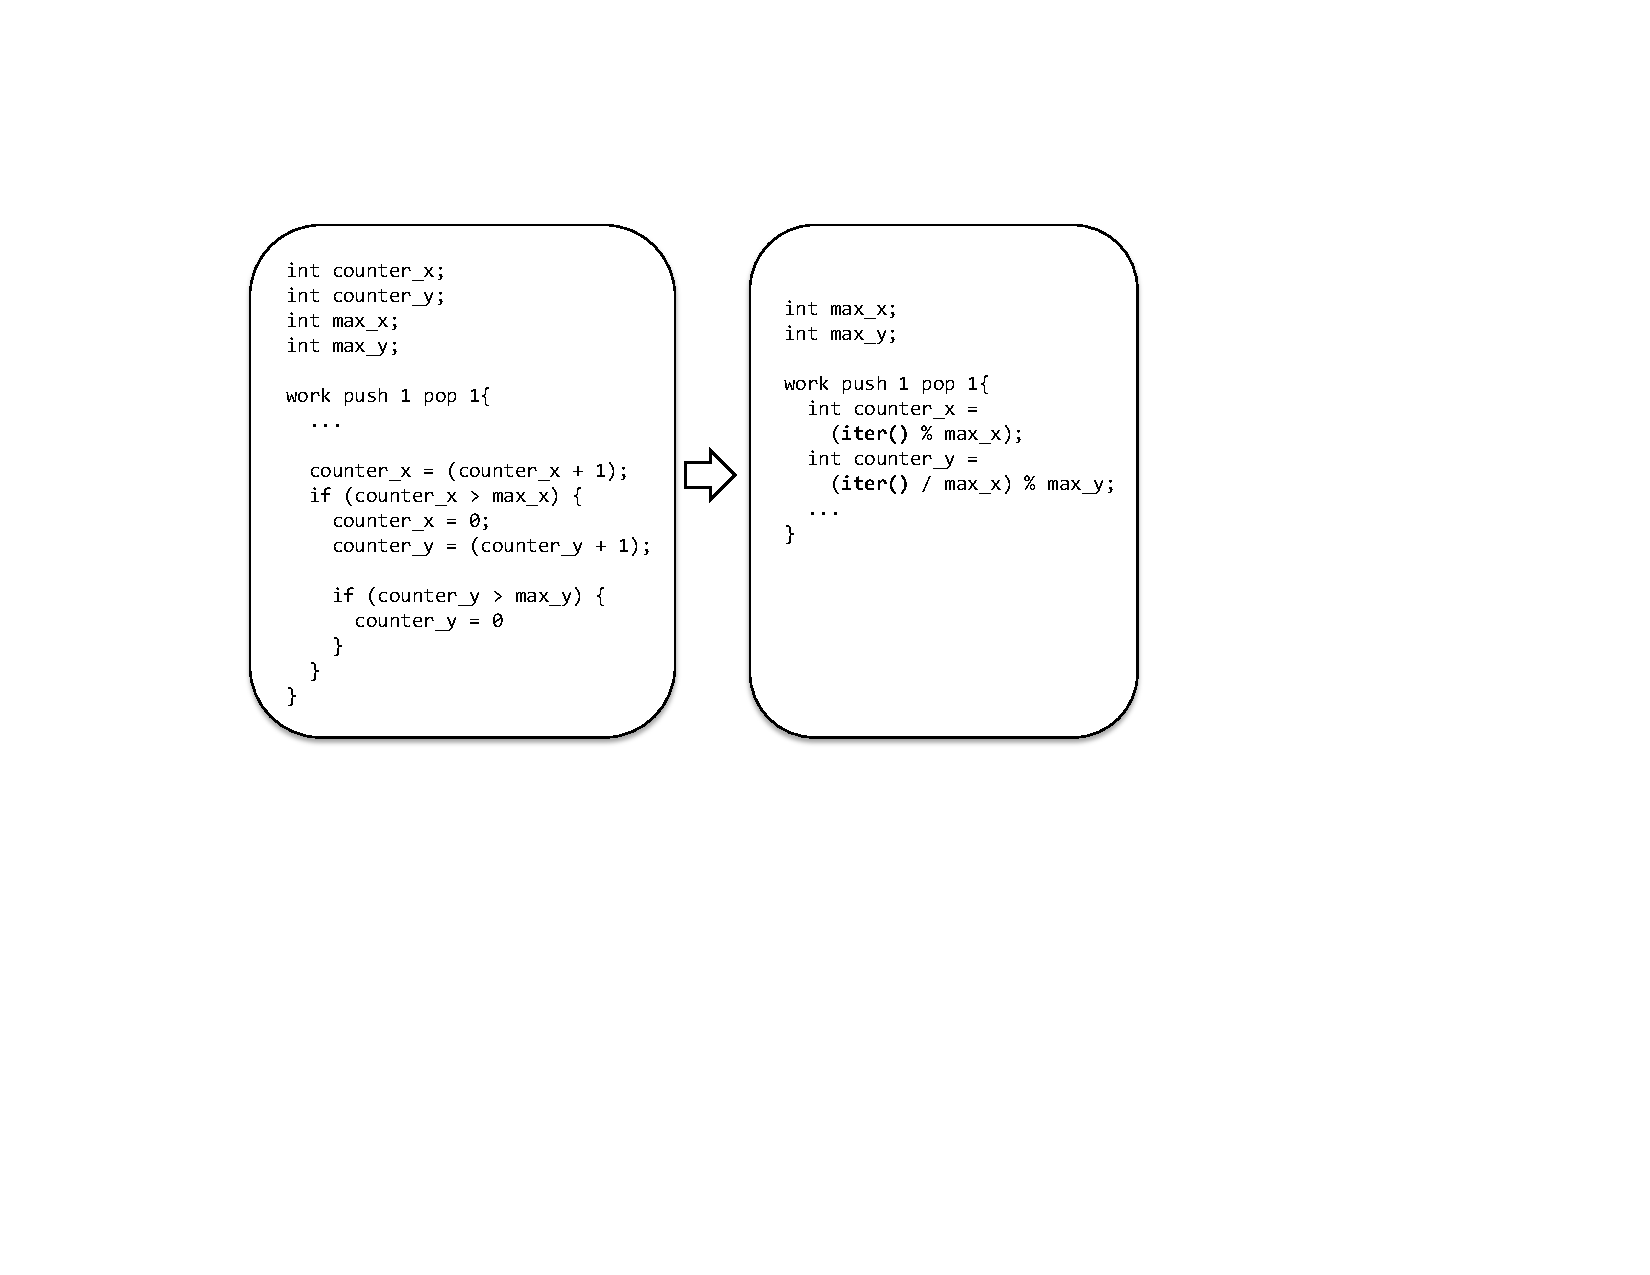
\includegraphics[width=3.3in]{figures/transformation3.pdf}
\caption{Translation of a filter with nested induction variables. \protect\label{fig:transform-after-twonested}}
\end{figure}


